Objectives : 
\begin{itemize}
    \item Present the rising velocity Vs. phi to demonstrate the 1/3 power law \citep{loisy2017buoyancy}
    \item Discus the common points and differences with bubbles and solid particles. 
    \item Discus the possible correlation between the shape /arrangement of the particles/flow lines with the rising velocity. 
    \item Present a proper definition of the drag force terms such as in \citet{wang2021numerical}. 
    \item Show that \citet{rusche2000effect}'s fit for the drag force is not adapted for our case and propose a new one
    \item All the references for teh Drag force terms are in \citet[chap 8]{morel2015mathematical} or in \citet{ishii2010thermo}
\end{itemize}
\todo[inline]{include fits of bubbly flow}
In this section we describe the influence of the \textit{Galileo} number and drop volume fraction on the interphase drag force. 

\begin{figure}[h!]
    \centering
    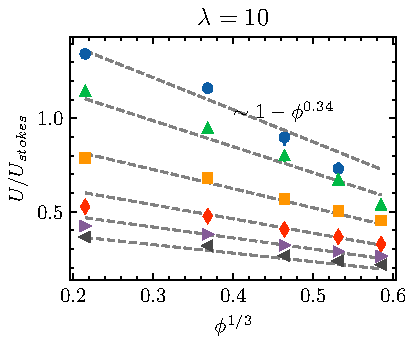
\includegraphics[height = 0.35\textwidth]{image/HOMOGENEOUS/fCA/UstokesGa_mu_r_0-1.pdf}
    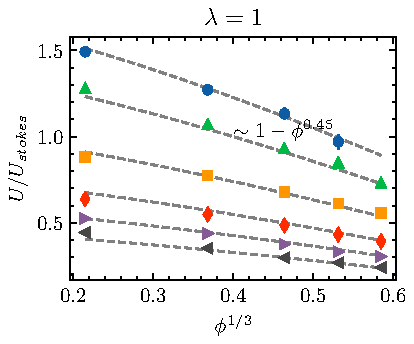
\includegraphics[height = 0.35\textwidth]{image/HOMOGENEOUS/fCA/UstokesGa_mu_r_1-0.pdf}
    \caption{Rising velocity divided by the rising velocity of an equivalent spherical drop in Stokes regime.($\bullet$) $Ga = 5\%$, ($\blacktriangle$) $Ga = 10\%$, ($\blacksquare$) $Ga = 50\%$ and ($\blacklozenge$) $Ga = 100\%$, 
    The dashed lines are the empirical funtions (left) $f(\lambda = 10) \sim (1 - \phi)^{-3.2}$
    (right) $f(\lambda = 1) \sim (1 - \phi)^{-2.6}$. notice that $f = 1 $correspond to the dillute stoke regime }. 
\end{figure}
    

\begin{figure}[h!]
    \centering
    
    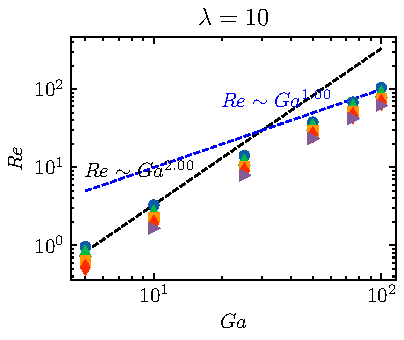
\includegraphics[height = 0.35\textwidth]{image/HOMOGENEOUS/fCA/Re_mu_r_0-1.pdf}
    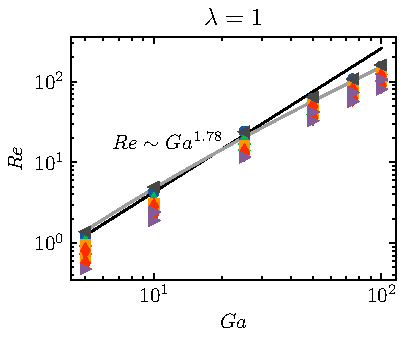
\includegraphics[height = 0.35\textwidth]{image/HOMOGENEOUS/fCA/Re_mu_r_1-0.pdf}
    
    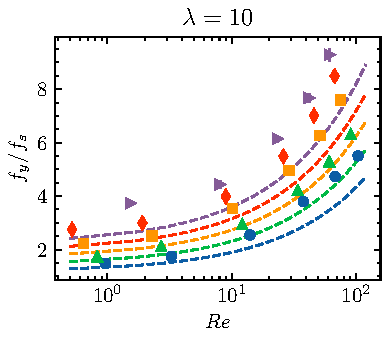
\includegraphics[height = 0.35\textwidth]{image/HOMOGENEOUS/fCA/Fstokes_mu_r_0-1.pdf}
    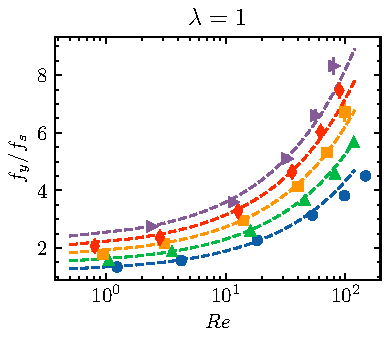
\includegraphics[height = 0.35\textwidth]{image/HOMOGENEOUS/fCA/Fstokes_mu_r_1-0.pdf}
    \caption{
        (middle) Reynolds number based on the averaged rising velocity.
    (bottom) Ensemble averaged drag force divided by the stokes drag force on spherical droplet of equivalent size.
    The symbols correspond to different volume fraction ($\bullet$) $\phi = 1\%$, ($\blacktriangle$) $\phi = 5\%$, ($\blacksquare$) $\phi = 10\%$, ($\blacklozenge$) $\phi = 15\%$ and ($\blacktriangleright$) $\phi = 20\%$.
    (dashed lines) empirical formulas }
\end{figure}
\tb{As discussed in previous study that
for spherical bubbles, as the gas fraction increases and the in-
teractions become more important, the bubbles tend to align
themselves in horizontal pairs, whose average rising velocity
is lower than that of an isolated bubbl}



In the stokes regime the drag force on a spherical droplet is, 
\begin{equation*}
    \textbf{F}_s
    =\pi \mu_f d (\textbf{u}_p - \textbf{u}_c) \left(\frac{2+3\lambda}{1+\lambda}\right)
\end{equation*}

Let the dimensionless drag force be a function of $\lambda$ $Re$ and $\phi$, expressed such that, 
\begin{equation}
    \textbf{f}_p(Re,\phi,\lambda)
    = 
    f_1^*(Re)
    f_2^*(\phi)
    \textbf{f}_s(\lambda)
\end{equation}
where $f_{1,2}$ are coefficient which limit tends to $1$ at low $\phi$ and low $Re$. 

To determine the $\phi$ dependency we base our study on the following analysis. 
In \cite[chapter 4]{ashgriz2011handbook} they stipulate that the last drops empirical were made form \citet{rusche2000effect} where they performed empirical fits on experimental datas. 
Some of which concerned droplets' sedimentation, were they stipulate that, 
\begin{align*}
    f_1^*(\phi) 
    &=1  + C_1 Re^{C_2}\\
    f_2^*(\phi) 
    &= e^{\phi K_1} + \phi K_2
\end{align*}

\todo[inline]{How to include more  physics ? }